\documentclass{beamer}

\begin{filecontents}{ref.bib}
    @inproceedings{struhr,
    author =	{V{\'a}clav Struh{\'a}r and Moris Behnam and Mohammad Ashjaei and Alessandro V. Papadopoulos},
    title =	{{Real-Time Containers: A Survey}},
    booktitle =	{2nd Workshop on Fog Computing and the IoT (Fog-IoT 2020)},
    year =	{2020},
    }
    @inproceedings{barletta2022achieving,
    title={Achieving isolation in mixed-criticality industrial edge systems with real-time containers},
    author={Barletta, Marco and Cinque, Marcello and De Simone, Luigi and Della Corte, Raffaele},
    booktitle={34th Euromicro Conference on Real-Time Systems (ECRTS 2022)},
    year={2022},
    organization={Schloss Dagstuhl-Leibniz-Zentrum f{\"u}r Informatik}
    }
    @inproceedings{abranches2019shimmy,
    title={Shimmy: Shared memory channels for high performance inter-container communication},
    author={Abranches, Marcelo and Goodarzy, Sepideh},
    booktitle={USENIX Workshop on Hot Topics in Edge Computing (HotEdge)},
    year={2019}
    }
    @inproceedings{dechev2006lock,
    title={Lock-free dynamically resizable arrays},
    author={Dechev, Damian and Pirkelbauer, Peter and Stroustrup, Bjarne},
    booktitle={OPODIS},
    volume={4305},
    pages={142--156},
    year={2006},
    organization={Springer}
    }
    @inproceedings{yun2013memguard,
    title={Memguard: Memory bandwidth reservation system for efficient performance isolation in multi-core platforms},
    author={Yun, Heechul and Yao, Gang and Pellizzoni, Rodolfo and Caccamo, Marco and Sha, Lui},
    booktitle={2013 IEEE 19th Real-Time and Embedded Technology and Applications Symposium (RTAS)},
    pages={55--64},
    year={2013},
    organization={IEEE}
    }
\end{filecontents}


\usepackage{wrapfig}
\usepackage{algpseudocode}
\usepackage{algorithm}
\usepackage[export]{adjustbox}
\usepackage{svg}

\usetheme{Boadilla}
\usecolortheme{dolphin}
\setbeamertemplate{navigation symbols}{}
\setbeamertemplate{sections/subsections in toc}[sections numbered]

\title[Containers Communications]{Design and Implementation of a Bandwidth Controlled Shared Memory Communication Model for Edge and Cloud Containers}
\author[MirSattarian, Afkar]{Sina MirSattarian \and Hossein Afkar}
\institute{University of Tehran}
\date{\today}

\begin{document}

\frame{\titlepage}

\begin{frame}
    \frametitle{Table of Contents}
    \tableofcontents[hideallsubsections]
\end{frame}

\section{Introduction}
\begin{frame}
    \frametitle{How Communicate containers together}
    \begin{itemize}
    	\item Container-to-Container Networking
    	\item Shared Volumes
    	\item Docker Networks
    	\item Service Discovery and Load Balancing
    	\item API-Based Communication
        \item Message Brokers (Publishers and Subscribers)
    \end{itemize}
\end{frame}

\begin{frame}
    \frametitle{Industry 4.0 and Container}
    Containers in Industry 4.0 are like small, self-contained boxes that hold different parts of the toy-making process. Each container has everything it needs to do its job, like the tools and materials required for a specific task.
\end{frame}

\begin{frame}
    \frametitle{Using containers in Industry 4.0 has several benefits}
    \begin{itemize}
    	\item Isolation
    	\item Portability
    	\item Efficiency
    	\item Standardization
    	\item Flexibility
    \end{itemize}
\end{frame}

\begin{frame}
    \frametitle{Edge Computing and Containers}
    In Edge Computing, we have many of these magic boxes called "containers."
    Each container has its own special ability, like analyzing data or
    controlling devices. But sometimes, one container alone can't do
    everything. That's when they need to communicate with each other
    and work together as a team.
\end{frame}

\begin{frame}
    \frametitle{Why Communication between containers in Edge Computing is important }
    \begin{itemize}
    	\item They can share information
    	\item They can work together
    	\item They can solve problems faster
    	\item They can adapt to changes
    \end{itemize}
\end{frame}

\begin{frame}
    \frametitle{We chose Local Communication between containers in Edge and Industry 4.0}
     When it comes to communicating between containers, it is important to
     understand that containers can be in different locations.
     Some containers may be running locally, while others may be running
     remotely or in a different place. In Edge Computing and Industry 4.0,
     the ability to communicate between these different types of containers
     is crucial.
\end{frame}

\begin{frame}
    \frametitle{How mixed critical environments can use a method of
    communication between real-time and isolated containers and it is good for it?}
    In a mixed critical environment, where there are both real-time
    and isolated containers, it is important to have a communication
    method that ensures both efficiency and reliability. One approach
    that can be beneficial in such cases is the use of a message-based
    communication system.
\end{frame}

\section{Design}

\begin{frame}
    \frametitle{Design Goals}
    \begin{itemize}
        \item Control Bandwidth of the memory.
        \item Reserve and repurpose unused bandwidth.
        \item Achieve Performance Isolation.
        \item Bounded Latency for communications.
    \end{itemize}
\end{frame}

\begin{frame}
    \frametitle{Bandwidth Conrtol}
    Ideas from this section is mostly influenced by the MemGuard paper
    \cite{yun2013memguard}.
    \begin{itemize}
        \item Performance Counters do not cover memory regions.
        \item Kernel Tracepoints apply their overhead in the kernel and
            therefore hurt determinism.
        \item Ask the user to count the accesses.
            \begin{itemize}
                \item Allocate a page.
                \item Store the metrics in that page with an RCU lock or a
                    mutex.
                \item Do it in the userlevel to avoid costly address space
                    switches.
            \end{itemize}
        \item Reset the counter at the hyperperiod
        \item If exceeding the bandwidth sleep the process and repeat.
    \end{itemize}
\end{frame}

\begin{frame}
    \frametitle{Reserve and repurpose unused bandwidth}
    Calculations are done before the write and read operations.
    \begin{itemize}
        \item Statically assigned bandwidth.
        \item Predicted bandwidth (Exponentially Weighted Moving Average).
        \item At the beginning of the priod is the minimum of the static and
            predicted bandwidth usages.
        \item Update the global budget accordingly.
        \item Then at the bandwidth exceed do this:
            \begin{itemize}
                \item Reclaim from the global if not exceeding static budget.
                \item Reclam a fixed $Q_{min}$ if not exceeding static budget.
                \item Maintain a global bandwidth remaining.
                \item If all shared regions used their budget or are finished
                    allocate budget from the global bandwidth.
            \end{itemize}
    \end{itemize}
\end{frame}

\begin{frame}
    \frametitle{Bound the latency}
    \begin{itemize}
        \item Real-time scheduled applications must be bound by time.
        \item Let the designer or scheduler assign a time budget to the
            communications. (May not be needed for the schedulability test.)
        \item Bail out of the communications on signal that we got from
            scheduler. (CLOCK\_THREAD\_CPUTIME\_ID is verified by reading
            kernel source code.)
    \end{itemize}
\end{frame}

\begin{frame}
    \frametitle{Proposed Design}
    \begin{figure}
        \centering
        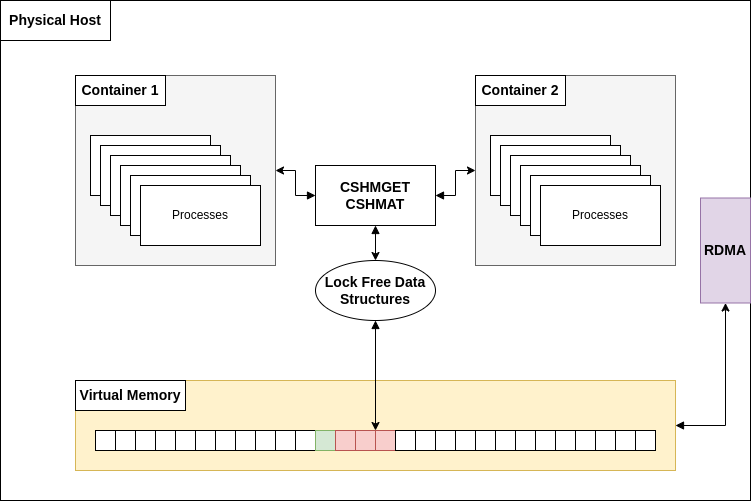
\includegraphics[width=0.8\textwidth]{dist.png}
        \caption{Simple Architecture Of The Proposed Design}
        \label{fig:desg}
    \end{figure}
\end{frame}

\section{Implementation}
\begin{frame}
    \frametitle{Implementations}
    Requirements for implementations:
    \begin{itemize}
        \item Edit the linux kernel syscalls.
        \item Choose a lock free data structure.
        \item Devise a test environment.
    \end{itemize}
\end{frame}

\begin{frame}
    \frametitle{Lock Free Vector Implementation}
    Non blocking algoritms can be categorized into following classification.
    \begin{description}[Obstruction Freedom]
        \item[Obstruction Freedom] Means that we gurantee progress as long
            there is no contention between thread.
        \item[Lock Freedom] Adds the requirement that the system as a whole
            makes progress even if there is contention.
        \item[Wait Freedom] Adds the requirement that every thread makes
            progress even if meets contention.
    \end{description}
\end{frame}

\begin{frame}
    \frametitle{Lock Free Vector Implementation}
    \begin{algorithmic}
        \Repeat
        \State $desc_{current} \gets vector.desc$
        \State $CompleteWrite(vector, desc_{current}.pending)$
        \If{$vector.memory[bucket]=NULL$}
        \State $AllocBucket(vector, bucket)$
        \EndIf
        \State $wop \gets new WriteDesc(At(desc_{current}.size)\^{}, elem,
        desc_{current}.size))$
        \State $desc_{next} \gets new Descriptor(desc_{current}.size + 1, wop)$
        \Until{$CAS(\&vector.desc, desc_{current}, desc_{next})$}
        \State $CompleteWrite(vector, desc_{next}.pending)$
    \end{algorithmic}
    This vector was implemented according to the paper by
    Dechev \cite{dechev2006lock}.
\end{frame}

\begin{frame}
    \frametitle{Development Environment}
    \begin{itemize}
        \item QEMU system virtualizor with kvm.
        \item debootstrap to create a debian image for sysroot.
        \item Linux 6.4.0 with standard config (Must be checked for docker
            support).
    \end{itemize}
\end{frame}

\begin{frame}
    \frametitle{Implemented System Calls}
    \begin{itemize}
        \item cshmget:
            \begin{itemize}
                \item Create the shared memory segment.
                \item Create and initialize the bookkeeping structures
            \end{itemize}
        \item cshmat:
            \begin{itemize}
                \item Attach the vm to shared segment.
                \item Handle event initializations if any.
            \end{itemize}
    \end{itemize}
    These syscalls were added in \textit{cshm.c} in ipc subsystem of the
    kernel.
\end{frame}

\begin{frame}
    \frametitle{Test Environment}
    \begin{itemize}
        \item Docker with:
            \begin{itemize}
                \item \textit{-ipc=host}
                \item \textit{-v /dev:/dev}
            \end{itemize}
        \item Simple C++ programs to do the communications.
    \end{itemize}
\end{frame}

\begin{frame}
    \frametitle{Results}
    \begin{itemize}
        \item Docker Kernel Requirements.
        \item Kernel Patch for the system calls.
        \item Lock free vector implementation.
        \item User level implementation of the bandwidth manager. \\
            (80\% Complete)
    \end{itemize}
\end{frame}

\begin{frame}
    \frametitle{Future Works}
    \begin{itemize}
        \item Handle RDMA:
            \begin{itemize}
                \item Real-time Ethernet.
                \item Handle Serialization and Error Handling.
                \item Handle Heterogeneous machines.
            \end{itemize}
        \item Less sophisticated design that could be fitted into a kernel
            module rather than a kernel patch.
        \item Handle ram access latency via cache coloring and ranks
            awareness.
        \item Compare the RDMA results with gRPC.
    \end{itemize}
\end{frame}

\begin{frame}
  \centering \Large
  \emph{Thank You For Your Attention}
\end{frame}

\begin{frame}{Reference}
    \bibliographystyle{apalike}
    \bibliography{ref.bib} 
\end{frame}


\end{document}
